\documentclass{article}\usepackage[]{graphicx}\usepackage[]{color}
%% maxwidth is the original width if it is less than linewidth
%% otherwise use linewidth (to make sure the graphics do not exceed the margin)
\makeatletter
\def\maxwidth{ %
  \ifdim\Gin@nat@width>\linewidth
    \linewidth
  \else
    \Gin@nat@width
  \fi
}
\makeatother

\definecolor{fgcolor}{rgb}{0.345, 0.345, 0.345}
\newcommand{\hlnum}[1]{\textcolor[rgb]{0.686,0.059,0.569}{#1}}%
\newcommand{\hlstr}[1]{\textcolor[rgb]{0.192,0.494,0.8}{#1}}%
\newcommand{\hlcom}[1]{\textcolor[rgb]{0.678,0.584,0.686}{\textit{#1}}}%
\newcommand{\hlopt}[1]{\textcolor[rgb]{0,0,0}{#1}}%
\newcommand{\hlstd}[1]{\textcolor[rgb]{0.345,0.345,0.345}{#1}}%
\newcommand{\hlkwa}[1]{\textcolor[rgb]{0.161,0.373,0.58}{\textbf{#1}}}%
\newcommand{\hlkwb}[1]{\textcolor[rgb]{0.69,0.353,0.396}{#1}}%
\newcommand{\hlkwc}[1]{\textcolor[rgb]{0.333,0.667,0.333}{#1}}%
\newcommand{\hlkwd}[1]{\textcolor[rgb]{0.737,0.353,0.396}{\textbf{#1}}}%
\let\hlipl\hlkwb

\usepackage{framed}
\makeatletter
\newenvironment{kframe}{%
 \def\at@end@of@kframe{}%
 \ifinner\ifhmode%
  \def\at@end@of@kframe{\end{minipage}}%
  \begin{minipage}{\columnwidth}%
 \fi\fi%
 \def\FrameCommand##1{\hskip\@totalleftmargin \hskip-\fboxsep
 \colorbox{shadecolor}{##1}\hskip-\fboxsep
     % There is no \\@totalrightmargin, so:
     \hskip-\linewidth \hskip-\@totalleftmargin \hskip\columnwidth}%
 \MakeFramed {\advance\hsize-\width
   \@totalleftmargin\z@ \linewidth\hsize
   \@setminipage}}%
 {\par\unskip\endMakeFramed%
 \at@end@of@kframe}
\makeatother

\definecolor{shadecolor}{rgb}{.97, .97, .97}
\definecolor{messagecolor}{rgb}{0, 0, 0}
\definecolor{warningcolor}{rgb}{1, 0, 1}
\definecolor{errorcolor}{rgb}{1, 0, 0}
\newenvironment{knitrout}{}{} % an empty environment to be redefined in TeX

\usepackage{alltt}
\usepackage{natbib}
\IfFileExists{upquote.sty}{\usepackage{upquote}}{}
\begin{document}

\title{Sense \& Sensibility Wordcloud}
\author{Ron Richardson}
\maketitle

\begin{abstract}
This article we construct a wordcloud using Jane Austen's book "Sense \& Sensibility", via the R package, janeaustenr.
\end{abstract}

\section{Introduction}
\textit{Sense \& Sensibility} is a novel was written in 1811 by Jane Austen\footnote{The novel was published anonymously.}. This article will show how to construct a wordcloud with the most commonly used words in the book.

\section{The Jane Austen Package}
There is a relatively new package for R called janeaustenr. This package contains all the novels written by Jane Austen \citep{Silge}. First, we need to install this package and load it in with the library command. Then, by calling the following function and store the result into a dataframe.

\begin{knitrout}
\definecolor{shadecolor}{rgb}{0.969, 0.969, 0.969}\color{fgcolor}\begin{kframe}
\begin{alltt}
\hlkwd{library}\hlstd{(janeaustenr)}
\hlstd{sns}\hlkwb{<-}\hlkwd{austen_books}\hlstd{()}
\end{alltt}
\end{kframe}
\end{knitrout}

\noindent This dataframe has two columns, one for each line in the novel, and another with the title of novel the line of text is from. Let's first filter using dplyr so we have only just the lines from \textit{Sense \& Sensibility}

\begin{knitrout}
\definecolor{shadecolor}{rgb}{0.969, 0.969, 0.969}\color{fgcolor}\begin{kframe}
\begin{alltt}
\hlkwd{library}\hlstd{(dplyr)}
\hlstd{sns}\hlkwb{<-}\hlstd{sns}\hlopt
  \hlkwd{filter}\hlstd{(book} \hlopt{==} \hlstr{'Sense & Sensibility'}\hlstd{)}
\hlkwd{print}\hlstd{(sns,} \hlkwc{n}\hlstd{=}\hlnum{20}\hlstd{)}
\end{alltt}
\begin{verbatim}
## # A tibble: 12,624 x 2
##                                                                      text
##                                                                     <chr>
##  1                                                  SENSE AND SENSIBILITY
##  2                                                                       
##  3                                                         by Jane Austen
##  4                                                                       
##  5                                                                 (1811)
##  6                                                                       
##  7                                                                       
##  8                                                                       
##  9                                                                       
## 10                                                              CHAPTER 1
## 11                                                                       
## 12                                                                       
## 13  The family of Dashwood had long been settled in Sussex.  Their estate
## 14   was large, and their residence was at Norland Park, in the centre of
## 15      their property, where, for many generations, they had lived in so
## 16    respectable a manner as to engage the general good opinion of their
## 17  surrounding acquaintance.  The late owner of this estate was a single
## 18   man, who lived to a very advanced age, and who for many years of his
## 19 life, had a constant companion and housekeeper in his sister.  But her
## 20       death, which happened ten years before his own, produced a great
## # ... with 1.26e+04 more rows, and 1 more variables: book <fctr>
\end{verbatim}
\end{kframe}
\end{knitrout}

\noindent Now we are ready for some data cleaning.

\section{Data Cleaning}
We would like to get the records that only contain the name and number of the chapter. To do this, we find any records that start with `Chapter`. We can use dplyr again, along with the R package called stringr.

\begin{knitrout}
\definecolor{shadecolor}{rgb}{0.969, 0.969, 0.969}\color{fgcolor}\begin{kframe}
\begin{alltt}
\hlkwd{library}\hlstd{(stringr)}
\hlstd{sns}\hlkwb{<-}\hlstd{sns}\hlopt
  \hlkwd{filter}\hlstd{(}\hlopt{!}\hlkwd{str_detect}\hlstd{(sns}\hlopt{$}\hlstd{text,} \hlstr{"^CHAPTER"}\hlstd{))}
\hlkwd{print}\hlstd{(sns,} \hlkwc{n}\hlstd{=}\hlnum{20}\hlstd{)}
\end{alltt}
\begin{verbatim}
## # A tibble: 12,574 x 2
##                                                                       text
##                                                                      <chr>
##  1                                                   SENSE AND SENSIBILITY
##  2                                                                        
##  3                                                          by Jane Austen
##  4                                                                        
##  5                                                                  (1811)
##  6                                                                        
##  7                                                                        
##  8                                                                        
##  9                                                                        
## 10                                                                        
## 11                                                                        
## 12   The family of Dashwood had long been settled in Sussex.  Their estate
## 13    was large, and their residence was at Norland Park, in the centre of
## 14       their property, where, for many generations, they had lived in so
## 15     respectable a manner as to engage the general good opinion of their
## 16   surrounding acquaintance.  The late owner of this estate was a single
## 17    man, who lived to a very advanced age, and who for many years of his
## 18  life, had a constant companion and housekeeper in his sister.  But her
## 19        death, which happened ten years before his own, produced a great
## 20 alteration in his home; for to supply her loss, he invited and received
## # ... with 1.255e+04 more rows, and 1 more variables: book <fctr>
\end{verbatim}
\end{kframe}
\end{knitrout}

\noindent We also want to remove the introduction text, as that is not relevant. We can find the positions of this by using the head() function to see what the line indexes are. Doing this, we see that the header ends at record 11, so we can redefine it to start at 12.

\begin{knitrout}
\definecolor{shadecolor}{rgb}{0.969, 0.969, 0.969}\color{fgcolor}\begin{kframe}
\begin{alltt}
\hlstd{sns}\hlkwb{<-}\hlstd{sns[}\hlnum{12}\hlopt{:}\hlnum{12562}\hlstd{,]}
\end{alltt}
\end{kframe}
\end{knitrout}

\section{The Wordcloud}
First off, we want break apart each line into indivual words, by using a tidytext function to un-nest tokens()

\begin{knitrout}
\definecolor{shadecolor}{rgb}{0.969, 0.969, 0.969}\color{fgcolor}\begin{kframe}
\begin{alltt}
\hlkwd{library}\hlstd{(tidytext)}
\hlstd{snsWords}\hlkwb{<-}\hlstd{sns}\hlopt
  \hlkwd{unnest_tokens}\hlstd{(word, text)}
\end{alltt}
\end{kframe}
\end{knitrout}

\noindent Now we want to remove any unimportant words, called stop words. These words include `the`, `and`, `a`, and several others. 

\begin{knitrout}
\definecolor{shadecolor}{rgb}{0.969, 0.969, 0.969}\color{fgcolor}\begin{kframe}
\begin{alltt}
\hlstd{snsWords}\hlkwb{<-}\hlstd{snsWords}\hlopt
  \hlkwd{filter}\hlstd{(}\hlopt{!}\hlstd{(word} \hlopt \hlstd{stop_words}\hlopt{$}\hlstd{word))}

\hlkwd{head}\hlstd{(snsWords)}
\end{alltt}
\begin{verbatim}
## # A tibble: 6 x 2
##                  book      word
##                <fctr>     <chr>
## 1 Sense & Sensibility    family
## 2 Sense & Sensibility  dashwood
## 3 Sense & Sensibility   settled
## 4 Sense & Sensibility    sussex
## 5 Sense & Sensibility    estate
## 6 Sense & Sensibility residence
\end{verbatim}
\end{kframe}
\end{knitrout}

\noindent The last step before building our wordcloud is to get a count of each word using dplyr.

\begin{knitrout}
\definecolor{shadecolor}{rgb}{0.969, 0.969, 0.969}\color{fgcolor}\begin{kframe}
\begin{alltt}
\hlstd{snsWordFreq}\hlkwb{<-}\hlstd{snsWords}\hlopt
  \hlkwd{group_by}\hlstd{(word)}\hlopt
  \hlkwd{summarize}\hlstd{(}\hlkwc{count}\hlstd{=}\hlkwd{n}\hlstd{())}

\hlkwd{head}\hlstd{(snsWordFreq)}
\end{alltt}
\begin{verbatim}
## # A tibble: 6 x 2
##        word count
##       <chr> <int>
## 1         1     1
## 2       200     1
## 3     7000l     1
## 4 abandoned     1
## 5 abatement     1
## 6 abbeyland     1
\end{verbatim}
\end{kframe}
\end{knitrout}

\noindent Finally, we can add the words and frequencies to the wordcloud function. Since there are so many unique words in the novel, we want to only include the words that occur more than 25 times.

\begin{knitrout}
\definecolor{shadecolor}{rgb}{0.969, 0.969, 0.969}\color{fgcolor}\begin{kframe}
\begin{alltt}
\hlkwd{library}\hlstd{(wordcloud)}
\hlkwd{wordcloud}\hlstd{(snsWordFreq}\hlopt{$}\hlstd{word, snsWordFreq}\hlopt{$}\hlstd{count,} \hlkwc{min.freq}\hlstd{=}\hlnum{25}\hlstd{)}
\end{alltt}
\end{kframe}
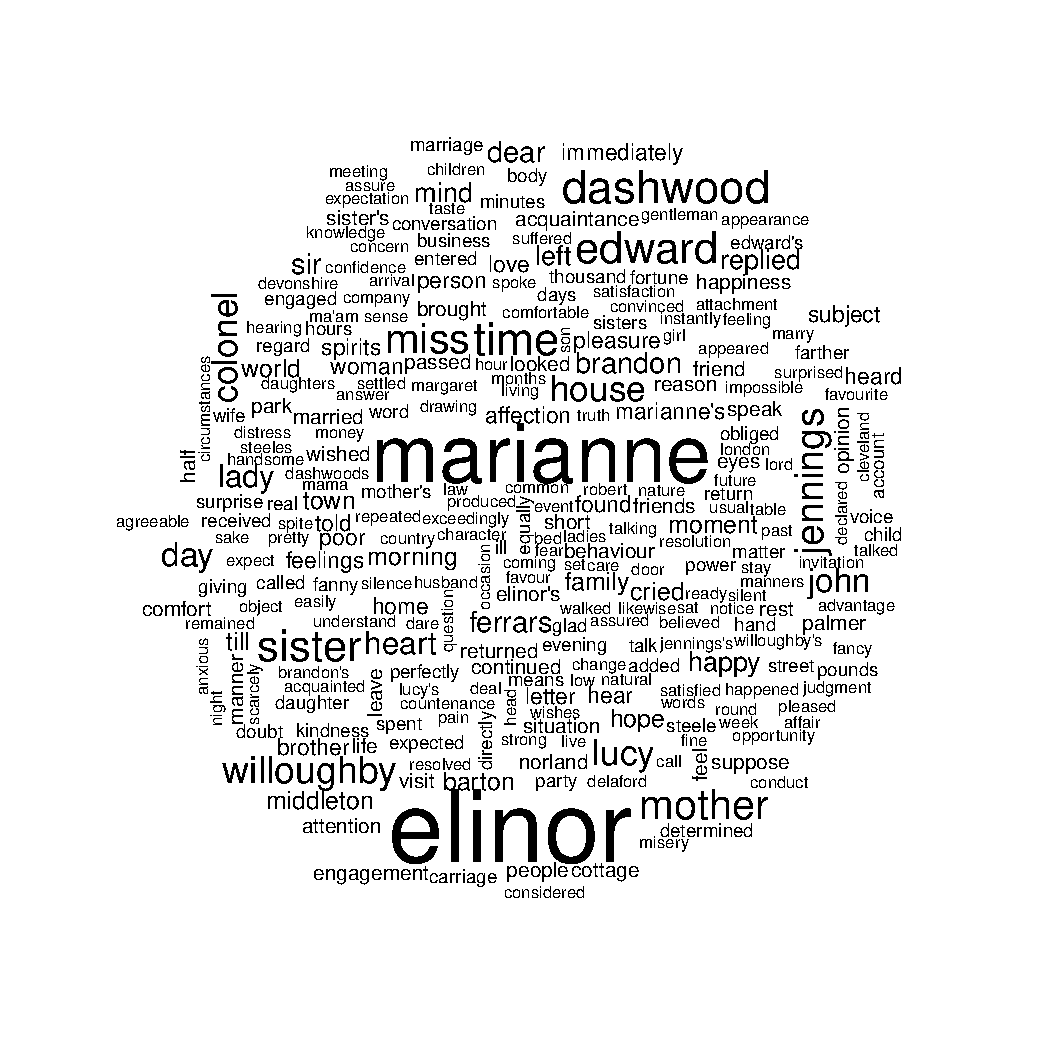
\includegraphics[width=\maxwidth]{figure/unnamed-chunk-8-1} 

\end{knitrout}


\bibliographystyle{apa}
\bibliography{janeausten}
\nocite{*}


\end{document}
